\ProvidesFile{chapters/ch-Motivation_Theory.tex}

\chapter{Motivation and Theoretical Overview}

%\section{Planck Units}
%The system of Planck units is defined in terms of the fundamental physical constants.
%In this system, many expressions in physics are simplified by setting the speed of light ($c$) and the reduced Planck's constant ($\hbar$) to unity.

\section{Reductionism and a Brief History of Particle Physics}
The reductionist approach of understanding nature by reducing it to its individual parts and studying the interactions between them, has been a central aspect of natural philosophy and scientific theory.
Well before there was evidence of the discreteness of matter, and despite human senses suggesting its continuity, ancient Greek philosophers Democritus and Leucippus introduced the concept of atoms as fundamental building blocks of matter in the fifth century B.C.
Ancient Greek atomism sought to reduce components of the cosmos to matter and empty space, propose that the fundamental constituents of matter were indivisible, and provide a natural explanation for the diversity of matter as resulting from atoms of different properties forming complex arrangements.
This early reductionist philosophy was remarkably well ahead of its time, and although ancient atomic theory and its concepts fell into obscurity after being rejected by later Greek philosophers including Aristotle, they were rediscovered by Enlightenment scientists in early 19th century and helped lay the foundation for modern atomic theory, which forms the basis for our understanding of the structure of matter and the nature of chemical reactions.

Since adopting the reductionist approach, the following 200 years resulted in unprecedented progress in the field of particle physics.
After discovering periodic trends in 1863, the Russian chemist Mendeleev published the first version of the periodic table in 1869, which organized chemical elements in a tabular arrangement based on patterns of chemical properties and atomic weight.
By the end of the 19th century, with the discoveries of the electron ($e$) by Thomson in 1897 and nuclear radioactivity by Becquerel in 1896, atoms were understood to not be indivisible and indestructible, and therefore could not be elementary constituents of matter.
In the early 20th century, Moseley revised the periodic table of elements after discovering atomic number, and this revision established a more accurate and consistent periodic table that led to better understanding of the electron structure of atoms.
Around the same time, Rutherford experimentally discovered the atomic nucleus and formulated the concept of the proton ($p$).
Some years later, to account for the missing mass discrepancy between measurements of atomic weight and atomic number, he also theorized the existence of neutrons.
With the discovery of the of the neutron ($n$) in 1932 by Chadwick, for a time it was thought that protons, neutrons, and electrons constituted fundamental particles.

The development of a quantum mechanical framework in the 20th century provided a deeper understanding of the behavior of atomic and subatomic particles that helped illuminate previously unexplained phenomena such as the atomic spectra and nuclear radioactivity.
In the 1930s, Fermi formulated a theoretical framework that described beta decay as the result of the weak interaction between subatomic protons, neutrons, and electrons.
The development of the quantum field theory of electrodynamics (QED) by Schwinger and Feynman in the 1940s and 1950s, provided a complete theoretical quantum framework for describing electromagnetism, which is responsible for phenomena such as electricity and light.
With the development of cosmic ray experiments in the 1940s and particle accelerator experiments in the 1950s, an extensive "zoo" of subatomic and subnuclear particles were discovered.
The formulation of the quark model by Gell-Mann in 1964, and the development of quantum field theory of chromodynamics (QCD) in 1973, elucidated that protons, neutrons, and many other species in the particle zoo, did not constitute fundamental particles, but instead were composed of combinations of elementary quarks bound together by a strong nuclear force.

\section{The Standard Model of Particle Physics}
The Standard Model (SM) of particle physics~\ref{Standard_Model} was first formulated in 1974.
The SM reduced the complex and diverse behavior of all atomic and subatomic particles to the elementary particles and the fundamental interactions between them. 
Elementary particles, described by their properties and quantum numbers (spin, electric charge, color charge, and  weak isospin), are understood to be point-like objects that are truly indivisible and without any substructure whatsoever.
The SM is a quantum field theory (QFT), defined mathematically by the local gauge symmetry group $SU(3) \otimes SU(2) \otimes U(1)$, that incorporates the strong, weak, and electromagnetic interactions.
Of the natural forces considered to be fundamental, only the gravitational force is not described among the others in a quantum field theory formulation.
\begin{figure}[!ht]
  \begin{center}
    \begin{tabular}{c}
        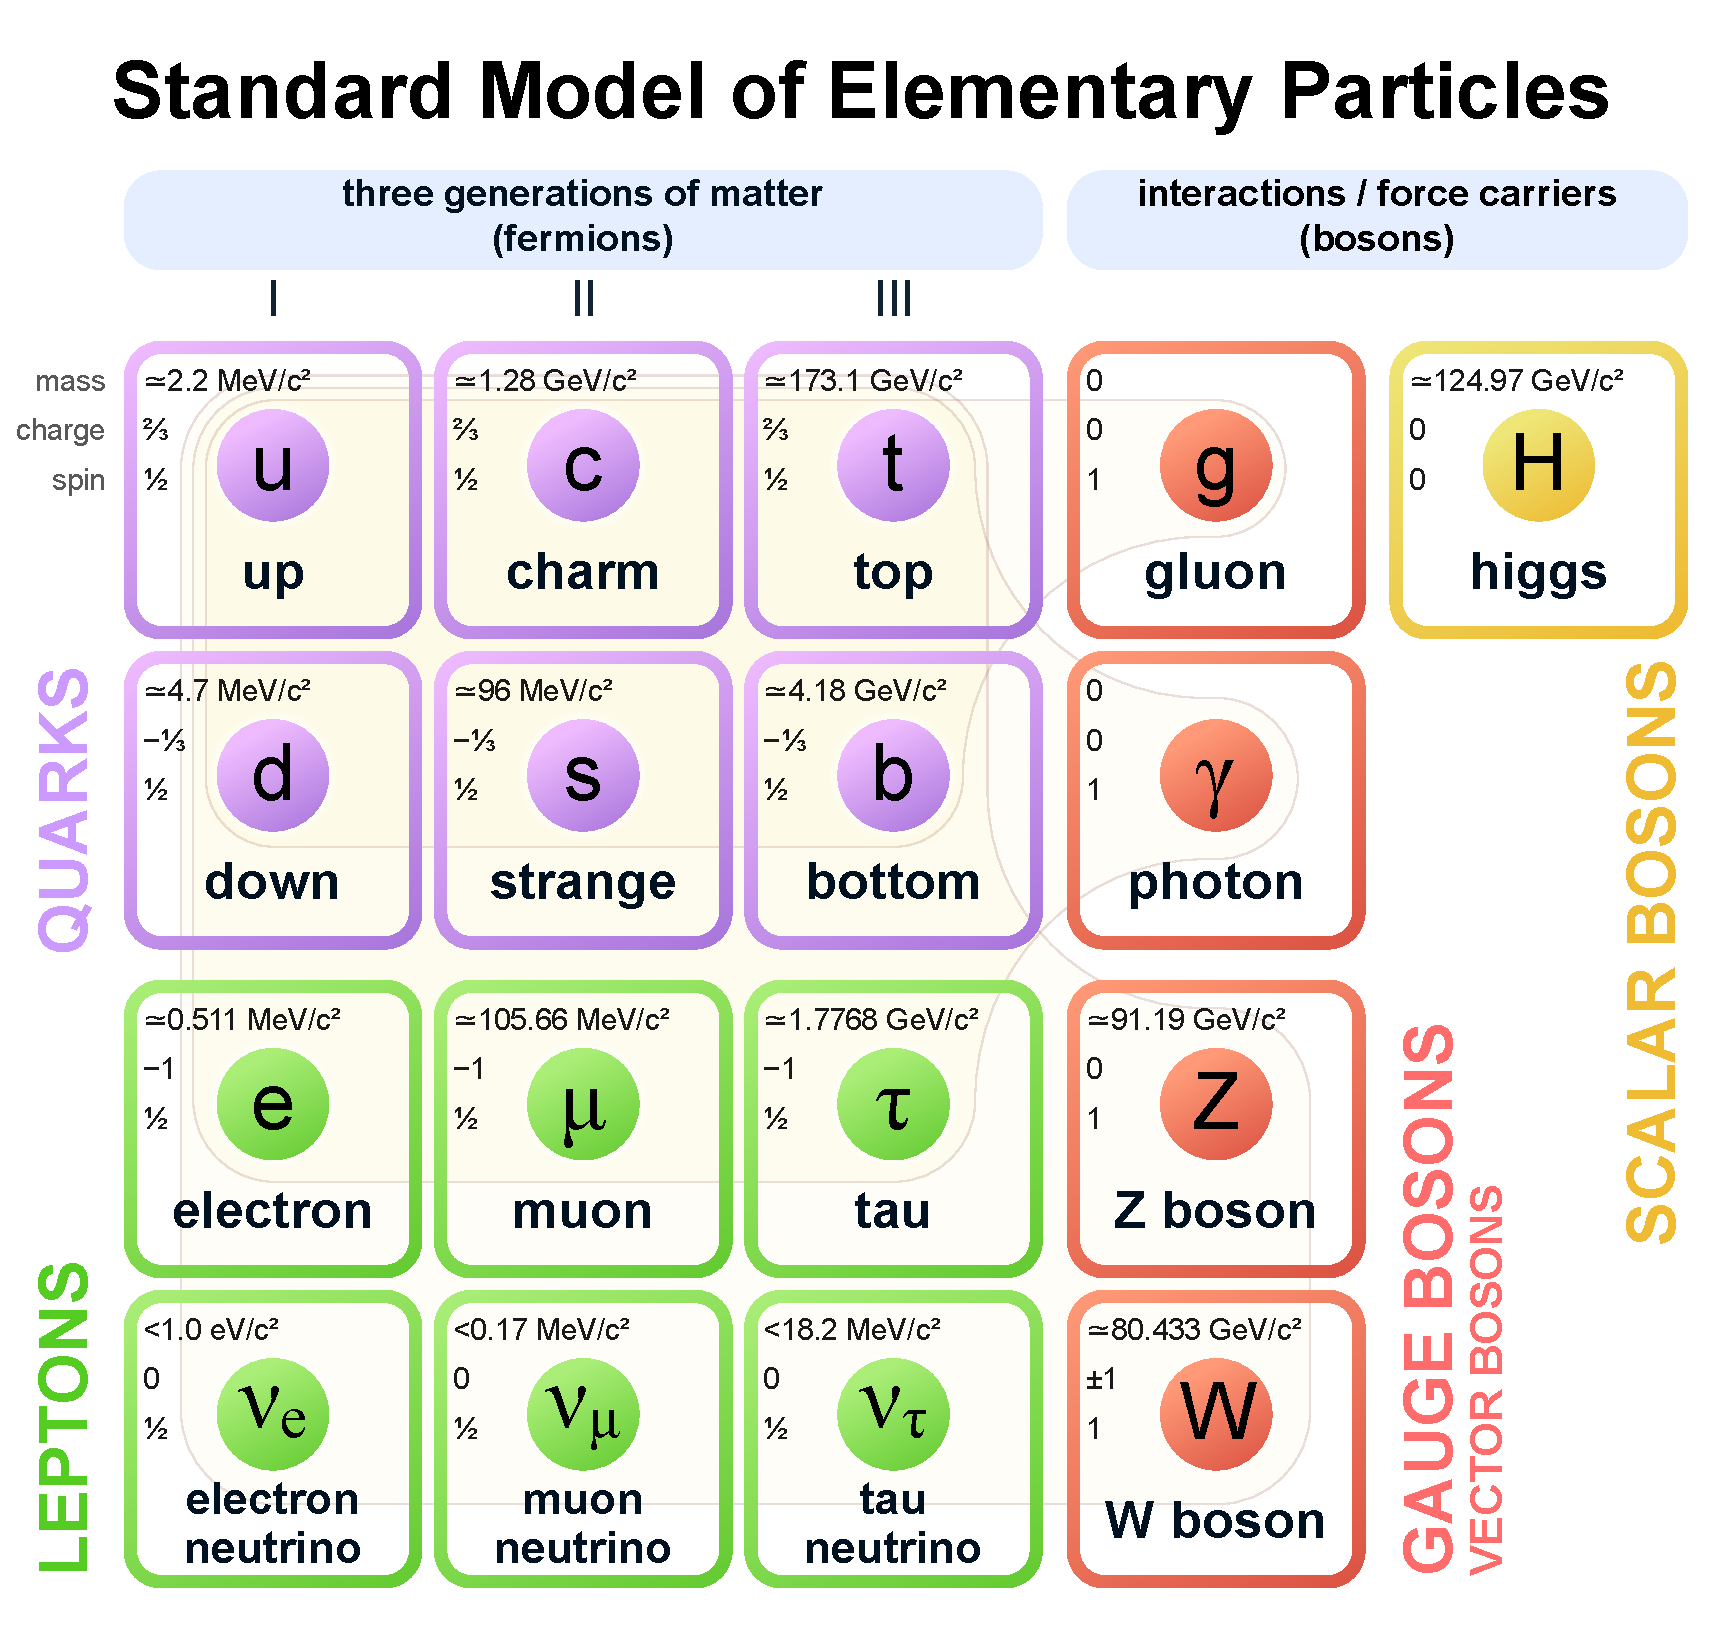
\includegraphics[width=0.75\textwidth]{fig_Theory/Standard_Model.pdf}
    \end{tabular}
    \caption{The Standard Model of Elementary Particle Physics
            }
    \label{Standard_Model}
  \end{center}
\end{figure}

\subsection{Fermions and Bosons}
In the SM, composite particles of matter are described in terms of their constituent elementary particles of half-integer spin, called fermions, which are particles of matter which are bound together by the exchange of fundamental, force-carrying particles of integer spin, called bosons. 

Fermions are further categorized into subgroups of quarks and leptons.
Leptons and quarks carry electric charge ($Q$) and therefore participate in the electromagnetic interaction.
Quarks additionally carry red ($R$), green ($G$), or blue ($B$) color charge, and so can also participate in the strong interactions.
Because of this property and the nature of QCD, quarks cannot exist in isolation, but instead can only be observed confined to colorless bound states called hadrons.
There are three so-called generations of fermions, and each generation is composed of both a pair of leptons and a pair of quarks, resulting in a total of twelve fermions: six quarks and six leptons.
Fermions of higher generations are more massive than those of the previous generation.
The up ($u$) and down ($d$) quarks, together with the electron ($e$) and electron neutrino ($\nu_e$) leptons, compose the first generation of fermions.
Both protons and neutrons are composed of different combinations of three up and down quarks; therefore, virtually all atomic matter is composed of only first generation fermions.
The second generation of fermions consists of the charm ($c$) and strange ($s$) quarks as well as the muon ($\mu$) and muon neutrino ($\nu_\mu$) leptons.
Finally, the third generation of fermions is composed of the top ($t$) and bottom ($b$) quarks (sometimes nicknamed truth and beauty), together with the tau ($\tau$) and tau neutrino ($\nu_\tau$) leptons.
The $e$, $\mu$, and $\tau$, referred to as "charged leptons", carry $Q = -1$, but the $\nu_e$, $\nu_\mu$, and $\nu_\tau$ neutrinos are electrically neutral.
The $u$, $c$, and $t$ quarks, referred to as "up-type," carry $Q = +\frac{2}{3}$, whereas the $d$, $c$, and $b$ quarks, referred to as "down-type," carry $Q = -\frac{1}{3}$.
Left-handed quarks and leptons additionally carry weak isospin ($I$ with third component $I_3$) and therefore participate in the weak interaction.
Left-handed charged leptons and down-type quarks carry $I_3 = +\frac{1}{2}$, while left-handed neutrinos and up-type quarks $I_3 = -\frac{1}{2}$.
Every fermion, i.e. denoted arbitrarily as $x$, has an anti-matter counterpart denoted $\Bar{x}$, that has the same mass as $x$, but opposite-signed quantum numbers.
The opposite-signed inversions of red, green and blue color charges are anti-red (cyan), anti-green (magenta) and anti-blue (yellow), respectively.

The fundamental interactions of the SM are described by exchange of mediating force-carrying spin-1 gauge bosons.
Mathematically, these mediators arise from the gauge field group generators of the symmetry groups $U(1)$, $SU(2)$, and $SU(3)$.
The SM also includes a spin-0 scalar boson that is associated with a scalar field responsible for breaking the weak isospin symmetry of the electroweak interaction.

\subsection{The Electromagnetic Interaction}
The photon ($\gamma$) is the massless and electrically neutral gauge boson that mediates the electromagnetic interaction between electrically charged particles.
The electromagnetic interaction is described by QED with gauge symmetry group $U(1)$.
The electromagnetic coupling, i.e. the fine structure constant $\alpha_{EM} \approx \frac{1}{137}$, is significantly small relative to unity.
For the given process, the momentum of mediating virtual photons depend on the energy scale, and therefore the coupling constant "runs," and the interaction becomes stronger (but still significantly smaller than unity) at higher energy scales.
As $\alpha_{EM} << 1$ even at higher energy scales, perturbative power series expansions in $\alpha_{EM}$ have proven to be extremely effective at explaining experimental results with QED.
Despite only providing approximate predictions, this effectiveness has made QED one of the most well-tested and successful theories in physics.

\subsection{The Weak Interaction}
The $W^\pm$ and $Z$ are massive gauge bosons that mediate the weak interaction between fermions carrying weak isospin ($I$ with third component $I_3$).
$W^\pm$ carries $Q = 0$, while $Z$ is electrically neutral.
Weak isospins of $I_3 = \pm 1$ ($I_3 = 0$) are carried by the $W^\pm$ ($Z$) bosons.
The $W^\pm$ and $Z$ boson masses are $\sim \SI{80.4}{\GeV}$ and $\sim \SI{91.2}{\GeV}$ respectively, resulting in their lifetimes, $\sim \SI{e-25}{\s}$, being incredibly short.
The short lifetimes limit the interaction ranges to be extremely small scales, as the distance these bosons can travel before decaying is very short.
The weak interaction is responsible for fermionic decay processes, such as nuclear radioactivity, is the only fundamental interaction that violates parity ($P$), charge conjugation parity ($CP$), and time-reversal ($T$) symmetries, and is described in the SM by gauge symmetry group $SU(2)$.
$Z$ bosons mediate the neutral weak interaction between same-flavor fermions, while $W^\pm$ bosons mediate the charged weak interaction between leptons of the same generation and can also flavor mix quarks of different generations.
Information about the conversion probabilities of flavor changing weak decays for quarks is encoded in the parameters of the Cabibbo-Kobayashi-Maskawa (CKM) matrix.

\subsection{The Strong Interaction}
Gluons ($g$) are massless gauge bosons that mediate the strong interaction between color charged particles.
The strong interaction is described by QCD with gauge symmetry group $SU(3)_C$.
While quarks (anti-quarks) carry color (anti-color) charge, gluons uniquely carry both color and anti-color charge, and therefore, gluons can interact with other gluons at trilinear and quartic self-interaction vertices.
There is a color octet of 8 different types of gluons, corresponding to 8 independent color state superpositions of the $3^2$ color/anti-color combinations.
One additional independent state exists mathematically, a color singlet carrying no color charge, but there is no experimental evidence for it and $SU(3)_C$ does not allow it.

The strong coupling $\alpha_S$ runs vigorously as the energy scale decreases, i.e. the interaction strength between quarks becomes stronger the further they are separated from each other.
This property of QCD results in color confinement, because before the energy between two separated quarks becomes arbitrarily large, a critical energy is reached for hadronization, in which a new quark/anti-quark pair is materialized from the energy of the mediating gluon.
Hadrons are classified by the flavor combinations of their valence quarks, but because quark interactions are mediated by gluons that can interact with themselves and split into quark/anti-quark pairs, there also exists a sea of virtual quarks and gluons within hadrons.
Protons and neutrons, colorless flavor combinations of three valence quarks, are categorized as baryons, whereas colorless flavor combinations of one valence quark and one valence anti-quark, such as pions and kaons, are categorized as mesons.
Experimental evidence for colorless flavor combinations of five valence quarks, categorized as pentaquarks, and colorless flavor combinations of two valence quarks and 2 valence anti-quarks, have also been reported in recent years.
Of all known hadrons, only the proton appears to be stable; with a mean life time constrained to be at least $10^34$ years, proton decay has never been observed.

Another consequence of the running of $\alpha_S$ is asymptotic freedom.
At higher and higher energy scales, $\alpha_S$ asymptotically approaches zero, i.e. quarks and gluons behave more like free particles at high energies.
At sufficiently high energy scales, such as those in hard scattering processes at hadron collider experiments, perturbative power series expansions in $\alpha_S$ become effective at explaining experimental results with QCD.

\subsection{The GWS Model, EWSB, and the BEH Mechanism}
At low energy energies, the electromagnetic and weak interactions are distinctly separate forces.
For energy scales beyond the unification energy $\sim$\SI{246}{\GeV}, electroweak theory unifies these two interactions into a single force described by a spontaneously broken Yang-Mills field with gauge symmetry group $SU(2)_L \otimes U(1)_Y$, generated by weak isospin ($I$) and weak hypercharge ($Y$).
In the Glashow-Weinberg-Salam (GWS) mopde, the $U(1)_Y$ group is mediated by a massless $B^0$ boson via the weak hypercharge field, and the $SU(2)_L$ group is mediated by massless $W^1$, $W^2$, and $W^3$ bosons via the weak isospin fields.
The subscript $L$ indicates that only left-handed fermion doublets carry isospin, while the right-handed singlets do not.

In the SM, the $\gamma$, $Z$, and $W^\pm$ bosons arise from the Brout-Englert-Higgs (BEH) mechanism spontaneously inducing electroweak symmetry breaking (EWSB) in the GWS model.
Mathematically, electric charge $Q = I_3 + \frac{1}{2} Y$ arises as a specific linear combination of weak isospin and hypercharge.
Electrically neutral $\gamma$ and $Z$ bosons arise from mixed states of the $B^0$ and $W^3$ bosons:
\begin{align}
\left(\begin{array}{c}
\gamma \\
Z^0
\end{array}\right)=\left(\begin{array}{cc}
\cos \theta_{\mathrm{W}} & \sin \theta_{\mathrm{W}} \\
-\sin \theta_{\mathrm{W}} & \cos \theta_{\mathrm{W}}
\end{array}\right)\left(\begin{array}{c}
B \\
W_3
\end{array}\right)
\label{}
\end{align}
where $\theta_{\mathrm{W}}$ is the Weinberg weak mixing angle.
Electrically charged $W^\pm$ bosons arise from linear combinations of the $W^1$ and $W^2$ bosons:
\begin{align}
W^{\pm}=\frac{1}{\sqrt{2}}\left(W_1 \mp i W_2\right).
\label{}
\end{align}

In the GWS model, local gauge symmetry prohibits mass terms in the Lagrangian for gauge bosons (Goldstone's theorem), but the $W^\pm$ and $Z$ bosons are experimentally known to have large masses.
To both resolve this discrepancy and induce EWSB, the BEH mechanism adds a complex scalar $SU(2)$ doublet field $\phi$ to the SM that permeates all of space:
\begin{align}
\phi=\left(\begin{array}{l}
\phi^{+} \\
\phi^0
\end{array}\right)=\frac{1}{\sqrt{2}}\left(\begin{array}{l}
\phi_1+i \phi_2 \\
\phi_3+i \phi_4
\end{array}\right)
\end{align}
with potential energy:
\begin{align}
V(\phi) = -\mu^2 \phi^{\dagger} \phi + \lambda\left(\phi^{\dagger} \phi\right)^2
\end{align}
The BEH potential, colloquially referred to as a Mexican-hat potential, has global $U(1)$ and $SU(2)$ symmetries.
The energy at the center of the potential is higher than at a ring of equivalent vacuum states with vacuum expectation energy $\langle\phi\rangle=\sqrt{\frac{\mu^2}{2 \lambda}} \equiv \frac{v}{\sqrt{2}}$ that breaks the electroweak gauge symmetry.
Without loss of generality, $\phi$ can be parameterized with an expansion around $v$, by introducing scalar field $h$, and with a unitary gauge transformation:
\begin{align}
\phi=\frac{1}{\sqrt{2}}\left(\begin{array}{c}
0 \\
v+h
\end{array}\right)
\end{align}
Of the original four degrees of freedom in the complex scalar $SU(2)$ doublet field, the electrically charged $\phi_1$ and $\phi_2$ are absorbed to generate mass terms in the Lagrangian for the $W^\pm$ bosons, while the electrically neutral $\phi_4$ term is absorbed to generate mass for the $Z$ boson.
The remaining electrically neutral $\phi_3$ is split into $v$ and the new field $h$, with quantum numbers $I_3 = \frac{-1}{2}$ and $Y = +1$ ($Q = 0$), which manifests as the physical Higgs ($H$) boson, a scalar boson that mediates interactions between the fermions and the BEH field, endowing them with mass proportional their Yukawa coupling constant $y_f$.
The Higgs boson was experimentally discovered in 2012 jointly by the CMS and ATLAS LHC experiments at CERN; Peter Higgs and François Englert received the 2013 Nobel Prize in Physics for their theoretical predictions, while Robert Brout passed away in 2011.

\section{Beyond the Standard Model}
The SM is a central pillar of modern particle physics, many of its predictions have been confirmed by innumerable experiments to exquisite precision, and is considered to be one of the most mature and successful theories in all of science.
Despite its success, there are a number of known physical phenomena that are not explained by the SM, and it is considered to be an effective theory up to some scale $\Lambda \approx \si{\TeV}$.
All theoretical and experimental investigations that are beyond the current understanding of the Standard Model of particle physics are collectively referred to as Beyond the Standard Model (BSM).

Following the example of electroweak unification, theoretical frameworks that aim to unify the strong and electroweak interactions into a single, unified force are referred to as Grand Unification Theories (GUT).
While the scale of electroweak unification is $\sim \SI{e2}{\GeV}$, the scale of grand unification is estimated to be $\sim \SI{e14}{\GeV} - \SI{e16}{\GeV}$.
Given the extreme energy requirements, it is unsurprising that no experimental evidence for GUT predictions have been found yet at energy scales accessible to modern particle accelerator experiments.

The the theoretical explanation for the experimental observation of neutrino oscillations predicts that the neutrino masses are non-zero.
However. the SM predicts that neutrinos should be massless particles. 

The discovery of the Higgs boson with mass $\sim \SI{125}{\GeV}$ has creating an inconsistency in the SM known as the "Heirarchy Problem."
Virtual loop corrections to the Higgs boson mass generate quadratic divergences.
Calculating a predicted Higgs boson mass compatible with the observed value requires unnatural fine-tuning, highlighting the likelihood of New Physics (NP) between the electroweak scale and the Planck scale, natural scale of quantum gravity.

The most glaring absence from the SM framework is the gravitational interaction between massive objects.
A theory that reduces all four physical interactions into a single, unified theory is colloquially referred to as the "Theory of Everything," and it is the holy grail of particle physics.
Einstein's general theory of relativity (GR) is a classical theory of gravitation that describes the force of gravity as resulting from the curvature of spacetime caused by the presence of massive objects.
All attempts to unify the SM and GR have failed, and the two are considered to be separate and incompatible theories.
A major focus of current theoretical physics research is centered around the formulation of a QFT that describes the gravitational interaction, but a common feature of these theories is that they are non-renormalizable.
Theories of quantum gravity predict the existence of a massless, spin-2 gauge boson dubbed the graviton.
Experimentally however, gravity is $\sim 10^{24}$ times weaker than the weak interaction, and the lack of experimental sensitivity makes it extremely difficult to verify the predictions of these theories.

There are astrophysical and cosmological observed physical phenomena as well that are not explained by the SM.
The asymmetry between the observed matter and anti-matter in the universe remains unexplained by the SM.
Based on the assumption that the universe started with equal quantities of matter and anti-matter, the conditions required for baryogenesis, i.e. the generation of a cosmological excess of baryons over anti-baryons, include baryon number violation, CP-violation, and charge conjugation symmetry ($C$) violation.
Sources of CP-violation in the SM via the weak interaction are not sufficient to account for the extreme asymmetry and baryon number is not violated whatsoever.
CP-violation via the strong interaction is mathematically allowed in the SM, but the relevant parameters have been inexplicably measured to be extremely small (strong CP problem).
Astronomical observations of gravitational lensing effects and in the velocity of rotation curves of spiral galaxies suggest that $85 \%$ of all observed matter in the universe is dark matter, an unknown form of matter that has its namesake in that it does not emit, absorb or reflect electromagnetic radiation, and thus can only be indirectly inferred through its gravitational effects on visible matter.
Although dedicated dark matter detection experiments exist that search for Weakly Interacting Massive Particles (WIMP), conclusive direct observation of dark matter WIMPs has not yet occurred.
Cosmological observations of galaxies also indicate that the expansion of space is accelerating.
The cause of this expansion is unknown, but it is attributed to an enigmatic form of energy, dubbed dark energy, that is thought to be responsible for $73 \%$ of the total energy density of the universe.

Many BSM extensions have been made that predict new elementary particles that, depending on their properties and stability, could explain dark matter.
Perhaps the most popular of these extensions is Supersymmetry (SUSY), which predicts the existence of superpartners for every fermion and boson in the SM by adding terms to the Lagrangian and make it symmetric with respect to matter and field-mediating particles.
SUSY can resolve the hierarchy problem by providing superpartner terms that cancel the quadratic divergences to the Higgs boson mass from heavy virtual particles.
Despite compelling arguments for why the predicted superpartners could be in reach of LHC experiments, the lack of experimental evidence for SUSY has led to a resurgence of interest in alternative BSM models to resolve these open questions.

SM Effective Field Theory (SMEFT) is a model-independent extension of the Standard Model which uses a systematic product expansion in terms of higher-dimensional operators to describe the effects of NP at higher energy scales.  
Due to its agnostic construction, SMEFT allows for a broad range of possibilities for NP, which is parameterized as coefficients of the operators in the expansion, referred to as Wilson coefficients.

